\chapter{Quanten-Teleportation\label{chapter:teleport}}
\lhead{Quanten-Teleportation}
\begin{refsection}
\chapterauthor{Max Obrist und Martin Stypinski}



\section{Einleitung}
Die Quantenteleportation beschreibt die Möglichkeit Quantenzustände über eine Distanz zu transportieren. Die Kernidee bei der Quantenteleportation ist nicht die Übertragung von Quanten, sondern viel mehr die Übertragung der Information. Ein Quantenzustand soll quasi von A nach B transportiert werden. Die Information soll über einen 'Informationskanal' übertragen werden, die Quanten an sich, da sie sehr schnell den Zustand ändern, aber werden im eigentlichen Sinne nicht übertragen.

\section{Problem}
\subsection{Klassische Kommunikation}
Angefangen bei der klassischen Kommunikation kann man die Informationsübertragung sehr einfach darstellen. Der Sender Alice verpackt seine Information eine Kiste. Diese wird mittels einem Speditionsunternehmen zu Bob transportiert. Bob öffnet die Kiste und findet die Information wieder. Die Kommunikation zwischen Alice und Bob konnte somit stattfinden. Dies ist sehr einfach und anschaulich erklärt und benötigt eine 'physische' Übertragung der Information. Einfacher ist es mit einem Faxgerät. Der Sender Alice faxt seine Meldung zu Empfänger Bob. Alice und Bob haben somit Informationen ausgetauscht.
\begin{figure}
\center
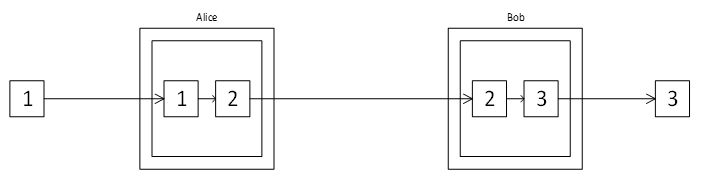
\includegraphics[width=0.75\textwidth]{teleport/image/classic_communication.png}
\caption{Klassische Kommunikation von Alice zu Bob.}
\label{Klassische Kommunikation}
\end{figure}
Die selbe "Uberlegung aus Quantenmechanischersicht betrachtet bringt aber ein wesentliches Problem. Die Meldung könnte nun auch von Alice und zu Charly gefaxt werden, jedoch wiederspricht diese Möglichkeit dem no-cloning Theorem. Quanten können nicht einfach kopiert werden. Es muss also eine andere Möglichkeit geben deren Zustand zu übertragen.
\section{L"osung}
\subsection{Das EPR Paar}
Der Effekt nach Einstein, Podolski und Rosen beschreibt ein Paradoxon, welcher zeigt, dass die Quantenmechanik gegen die Lokalität verstösst. (referenz paper hier). Dies hat zur Folge, dass zwei Teilchen eine Wechselwirkung eingehen können ohne in klassisch physikalischer Nähe zu liegen. Diese zwei Teilchen in Wechselwirkung nennt man auch EPR-Paar. Eine weitere Bedinnung stellt sich nun an das EPR-Paar um die Quantenteleportation möglich zu machen. Es wird ein sogenanter verschränkter Zustand benötigt. Ein verschränkter Zustand liegt vor, wenn sich der Zustand des Systems durch einen gemeinsamen Zustand beschreiben lässt, nicht aber durch die Ansammlung einzelner Teilchenzustände. Diese Bedinnung ermöglicht das spätere Auslesen.
\subsection{Teleportation}
Die Grundlagen sind geschafen um ein Qbit von Alice zu Bob zu übertragen. Nenen wir das Qbit $ \left|\psi\right\rangle_\mathrm A $ dieses lässt sich wie folgt darstellen:
\begin{align*}
\left|\psi\right\rangle_\mathrm A = \alpha \left|0\right\rangle_\mathrm A + \beta\left|1\right\rangle_\mathrm A
\end{align*}
Weiter gilt, dass der Betrag von $ \left|\psi\right\rangle_\mathrm A$ 1 ist. Somit ist der Gedanke naheliegend, dass bei der 'Bestimmung' von $\alpha$ oder $\beta$ die andere Komponente berechenbar ist. Durch die EPR Bedinnung ist auch ersichtlich, dass das Qbit $ \left|\psi\right\rangle_\mathrm B $ in Wechselwirkung mit A steht. Da B komplementär zu A ist, folgt daraus:
\begin{align*}
\left|\psi\right\rangle_\mathrm B = \beta \left|0\right\rangle_\mathrm A + \alpha\left|1\right\rangle_\mathrm B
\end{align*}
Es ist nun ersichtlich, dass mit der Messung einer Grösse in A die komplementäre Grösse in B beeinflusst wird.
% TODO BELL STATES!
\section{Anwendung}
	\begin{itemize}
		\item{\textbf{Quantencomputer} \\
			In einem Quantencomputer kann die Übertragung der Zustände zwischen einzelnen Komponenten von zentraler Bedeutung sein, dies könnte mittels der Quantenteleportation gelöst werden.
		}
		\item{\textbf{Quantenkryptographie} \\
			Das no-cloning Theorem besagt, dass die Zustände  nicht nur nicht kopiert werden können, sondern dass diese auch nicht einfach ausgelesen werden können. Sobald eine Messung erfolgt beeinflusst diese die Quantenzustände und die Information die übertragen werden soll ist somit verändert.
		}		
	\end{itemize}
\printbibliography[heading=subbibliography]
\end{refsection}